\documentclass[12pt,letterpaper,titlepage]{article}

\usepackage[utf8]{inputenc}
\usepackage{amsmath}
\usepackage{amsfonts}
\usepackage{amssymb}
\usepackage{array}
\usepackage[margin=2.5cm]{geometry}
\usepackage{graphicx}
\usepackage[section]{placeins}
\usepackage{rotating}
\usepackage{hyperref}
\usepackage{textcomp}

\renewcommand{\arraystretch}{1.05}


\author{Nathan Minor}
\title{Trupanion Data Scientist Candidate Homework}


\begin{document}

	\maketitle
 
		\begin{center}
			For Luke, the truest companion.
		\end{center}
		\newpage	
	
	\tableofcontents
	
	\newpage
	\section{Estimating Customer Value}
		
		One possible way to measure the remaining value of a policy, $p \in \mathbf{P}$, is to compute the difference between the sum of premiums paid, $\phi_p$ and the sum of claims paid, $\gamma_p$, over a given year. Here, $\mathbf{P}$ denotes the set of all policys held by the insurance company. The value of this difference, $\Lambda_p$, yields  the amount contributed by this policy to yearly profits. Below is a representation of this relationship:
		\begin{equation} \label{eq:Lambda_p}
			\Lambda_p = \phi_p - \gamma_p
		\end{equation}
		Instead of using this difference $\Lambda_p$ to analyze the remaining value of the policy $p$, weight $\omega_p$ and buoyancy $\beta_p$ measures can be calculated as follows:
		\begin{equation} \label{eq:omega_p}
			\omega_p = \frac{\gamma_p}{\sum\limits_{p \in \mathbf{P}}{\gamma_p}}
		\end{equation}
		\begin{equation} \label{eq:beta_p}
			\beta_p = \frac{\phi_p}{\sum\limits_{p \in \mathbf{P}}{\phi_p}}
		\end{equation}		
		Notice that for any $p \in \mathbf{P}$, it is apparent that $0 \leq \omega_p < 1$ and $0 < \beta_p < 1$. The weight of a policy, $\omega_p$ , is an expression of what fraction of the total claims paid out went to this policy. Similarly, the buoyancy of a policy, $\beta_p$, reflects what fraction of the total premiums collected were contrinuted by this policy. Calculating the difference between buoyancy and weight yields the net buoyancy of a policy:
		\begin{equation} \label{eq:Psi_p}
			\Psi_p = \beta_p - \omega_p
		\end{equation}		
		Positive values of $\Psi_p$ corresponds to a higher normalized value of contribution to the capital available for paying claims in comparison to the normalized value of depletion on that same capital. Negative values of $\Psi_p$ corresponds to a higher normalized value of depletion on the capital available for paying claims in comparison to the normalized value of contribution to that same captial. The net buoyancy of a policy provides greater insight into how this policy both contributes to and depletes from the overall capital of the insurance company.
		
		
				 
	\newpage
	\section{Predicting Policy Payouts (option b)}
		
		\subsection{Background}
		
			\subsubsection*{Prompt}
			Using the example data from 2016, provided in "ClaimLevel.csv," build a model to predict the future claims paid out per policy in the month of January, 2017. The output of the model should be an estimated dollar amount paid out for each policy.
			
			\subsubsection*{Problem Overview}
			The problem set forth by this prompt presents a classic example of mathematical modelling: predicting future behavior based on past knowledge. In this case, data on claims paid out during 2016 will be used for past knowledge, and estimated dollar amount paid out for January of 2017 will be the future behavior that the model will be predicting.
			
			\subsubsection*{Data Overview}
			The data table provided in the \emph{ClaimLevel.csv} file is structed as follows. Each row in the table is a vector representing four values for a claim made against a policy. These values represent \emph{PolicyId, ClaimDate, ClaimedAmount, PaidAmount} for each claim made against a policy in 2016. An example of a segment of the data table is represented below:
			
			\begin{figure}[!ht]
				\centering
				\begin{tabular}{|c|c|c|c|}
					\hline
					PolicyId & ClaimDate & ClaimedAmount & PaidAmount \\
					\hline
					148971	& 2016-02-11	& 924.39	& 814.27 \\
					566332	& 2016-01-20	& 155.43	& 0 \\
					221990	& 2016-01-14	& 1579.88	& 1136.89 \\
					568257	& 2016-01-13	& 220.33	& 39.89 \\
					403218	& 2016-01-08	& 46.11		& 13.87 \\
					769941	& 2016-01-25	& 152.38	& 0 \\
					423993	& 2016-01-24	& 142.32	& 128.09 \\
					717214	& 2016-01-12	& 171.52	& 0 \\
					248362	& 2016-01-08	& 125.62	& 0 \\
					89779	& 2016-01-04	& 24.88		& 0 \\
					\hline
				\end{tabular}
				\caption{The table above represents a segment from the raw claim level data in \emph{ClaimLevel.csv}.} 	
				\label{tab:exampleData}
			\end{figure}	
			\FloatBarrier

			Included next are some standard charts used to analyze and understand the distribution of the data. First is a histogram of the amounts paid out on claim. This histogram shows that, in comparison to a normal distrubution, the distribution of data for the amount paid on claim is skewed right with a mean of \$96.80 and median of \$21.26, amount paid on a claim. Being skewed right means that measures of center (mean and median), are still valid for understanding an average or typical value for the data. However, some measures of spread, specifically standard deviation, no longer accurtely describe the asymmetry the data. Using quantiles provides a better understanding of the symmetry of the data. For all the claims filed in 2016, at least 25\% cost \$0,  50\% cost \$21.26 or less, 75\% cost \$73.97 or less, 95\% cost \$384.89 or less, and 99\% of all claims paid out in 2016 cost \$1494.30 or less. These quantiles provide excellent insight into the distribution of amounts paid on claims, for another visual representation of the density of the amounts paid out on claims filed in 2016, see Figure \ref{fig:amountByPolicyId_2016}.
			
			\begin{figure}[!ht]
			\centering
				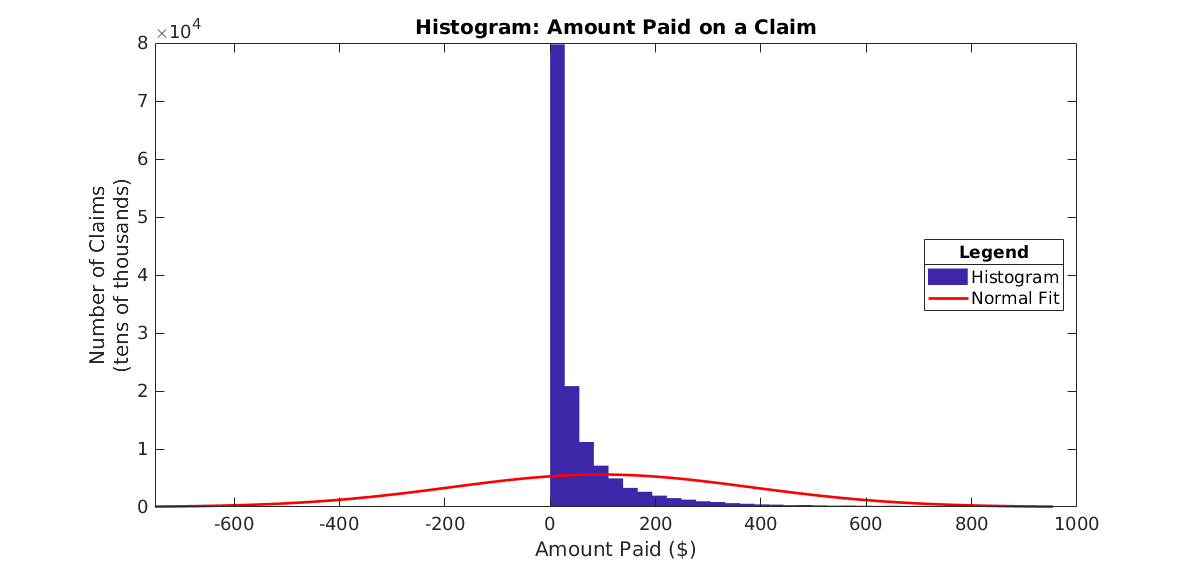
\includegraphics[scale=0.4]{hist_amountPaid.png}
				\caption{A histogram of the amounts paid out on a claim. Notice the right skew in comparison with a normal distribution centered at the same mean. Also, take note that, with a right-skewed distribution, the mean (\$96.80) is \emph{greater than} the median (\$21.26).}
				\label{fig:hist_amountPaid}
			\end{figure}
			\FloatBarrier
			
			The following histogram shows the number of claims paid, binned per month. This is an approximately uniform distribution from which we can quickly approximate that the total number of claims paid per month fell between 10,000 and 14,000, with an approximate mean of 12,000. This information is insightful, and could be useful with future model variations, but ultimately not useful for the further purposes of this report.
			
			\begin{figure}[!ht]
			\centering
				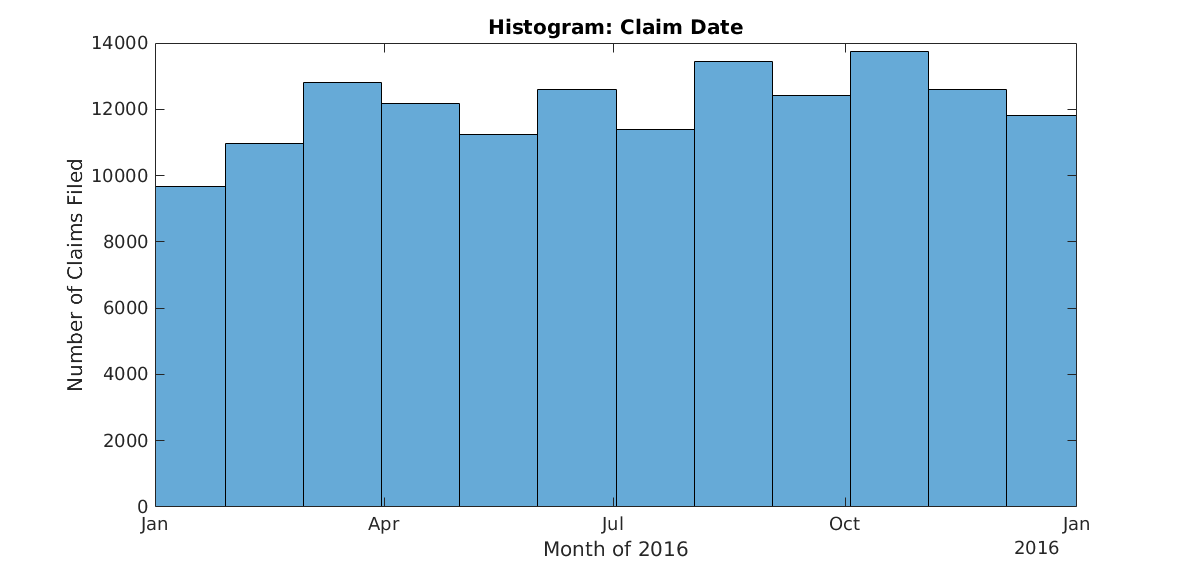
\includegraphics[scale=0.4]{hist_claimDate.png}
				\caption{A histogram of when claims were made, with bins corresponding to each month. Notice the uniform distrubution with an approximate minimum, mean, maximum number of claims per month of 10,000, 12,000, and 14,000, respectively.}
				\label{fig:hist_claimDate}
			\end{figure}
			\FloatBarrier
		
		\subsection{Assumptions} \label{sec:assumptions}
			
			\subsubsection*{Periodic Behavior}
			Allowing for the assumption that visits to the veterinary clinic are cyclical and repetetive, allows for a periodic approximation to be implemented to calculate a probability associated with when the next payout on a policy can be expected. This timing probability is used to attenuate the reversion to the mean calculation. 
		
			\subsubsection*{Reversion to the Mean}
				According to Wolfram's Web Resource, MathWorld, "reversion to the mean, also called regression to the mean, is the statistical phenomenon stating that the greater the deviation of a random variable from its mean, the greater the probability that the next measured variate will deviate less from its mean." (Weisstein, Eric W. "Reversion to the Mean." From MathWorld--A Wolfram Web Resource. http://mathworld.wolfram.com/ReversiontotheMean.html) The following model will use this concept for the implementation of restoring the next monthly paid amount on the policy closer to the mean monthly paid amount on that policy (or its cluster).
				
			\subsubsection*{Diverse Data}
			Since the data used for this forecasting model represents a wide client base with many different possible groupings, or clusterings, based on defining features or characteristics of each policy. A clustering algorithm can be used to help improve the accuracy of the overall model. See \emph{Further Work} (section \ref{sec:furtherWork}) for more details.
		
		\subsection{Definitions}
			\subsubsection{Terms}
				Defined below are terms used throughout the rest of this document. Before going into any further details about this forecasting model, let us define some terms.
				\begin{itemize}
					\item \emph{Policy Id} A number associated with a particular policy.
					\item \emph{Claim Date} The date a claim was filed against a policy.
					\item \emph{Claimed Amount} The amount asked for on the claim filed against a policy.
					\item \emph{Paid Amount} The amount pait out against the claim filed on a policy.				
				\end{itemize}
				
			\subsubsection{Variables}
				Next to define are specific variables and their usages.
				\begin{itemize}
					\item \emph{Independent Variable} As in most modeling scenarios, time $t$, will be the independent variable. For the purposes of this model, time will be in months as follows: $t = 0 \rightarrow $ Jan 2016 $, t = 1 \rightarrow $ Feb 2016 $,..., t = 11 \rightarrow $ Dec 2016 $, t = 12 \rightarrow $ Jan 2017.
				
					\item \emph{Response Variable} This model is predicting $x_p(t) = $ the amount paid against a policy Id, $p$, for a given month, $t$. 
				
					\item \emph{Other Factors} Some other measures related to a policy Id that will be used to calculate a prediction are as follows:
						\begin{itemize}\label{eq:ofEq}
							\item[(a)] $\overline{x_p} = \text{ mean monthly amount paid against policy Id, } p$
							
							\item[(b)] $\overline{t_p} = \text{ mean time between amounts paid against policy Id, } p$
							
							\item[(c)] $\sigma_{t_p} = \text{ standard deviation of time between amount paid against policy Id, } p $
							
							\item[(d)] ${t_p}^{*} = \text{ previous month an amount was paid against policy Id, } p$
						\end{itemize}
				 \end{itemize}

				
			\subsubsection{Equations} Now onto some important equations.
			
				\begin{enumerate}
					\item{Error from the Mean (normalized to the range} 
						\begin{equation} \label{eq:efmEq}
							e_p(t) = \frac{x_p({t_p}^*) - \overline{x_p}}{\max{x_p} - \min{x_p}}
						\end{equation}
						
					\item{Time Since Last Amount Paid (z-score)}
						\begin{equation} \label{eq:tZscoreEq}
							z_p(t) = \frac{\Delta{t} - \overline{t_p}}{\sigma_{t_p}} = \frac{(t - {t_{p}}^*) - \overline{t_p}}{\sigma_{t_p}}
						\end{equation}
						
					\item{Timing Probability} 
						\begin{equation} \label{eq:timeProbEq}
							Q_p(t) = 
							\begin{cases}
								0	
									& \text{if $|z_t| > 2 \sigma_{t_p}$} \\
							
								\frac{|z_t| - 2 \sigma_{t_p}}{2 \sigma_{t_p}} 									
									& \text{otherwise} \\
							
							\end{cases}
						\end{equation}
						
					\item{Payout Prediction}
						\begin{equation} \label{eq:predEq}
							X_p(t) = Q_p(t) (\overline{x_p} (1 - e_p(t)))
						\end{equation}
				\end{enumerate}
								
		\subsection{Computer Model}
		Originally, this computer model was written as a console application in Java\texttrademark \; for the ease of debugging and testing, as well as for the simplicity of implementation. In the \emph{Futher Work} section (\ref{sec:furtherWork}) there are more details about plans for scaling and expanding this computer model.
			
			\subsubsection{Procedure} \label{sec:procedure}
				\begin{enumerate}
					\item Retrieve raw claim level data from CSV file: "ClaimLevel.csv" (See \emph{RetrieveData} method in \emph{DataHandling} class)
					
					\item Aggregate claim level data to monthly summaries for each policyId. (See \emph{CalculatePolicySummaries} method in \emph{ForecastEngine} class)
					
					\item Aggregate monthly summaries to overall payout summaries for each policyId, calculating other factors \ref{eq:ofEq}. (See \emph{CalculatePolicySummaries} method in \emph{ForecastEngine} class)
					
					\item For a given month, calculate the predicted payout per policyId using the results from payout summaries in previous step.  (See \emph{CalculatePredictions} method in \emph{ForecastEngine} class)
					
					\item Save predictions, and values used for predictions to a CSV file. (See \emph{SavePredictions} method in \emph{DataHandling} class)
					
					\item Repeat steps 4 for each month Jan16-Jan17, inclusive.  (See major \emph{for} loop in \emph{main} method within the \emph{Main} class, aka the entry point for the execution of this program)
				\end{enumerate}
				
				
			\begin{figure}[!ht]
			\centering
				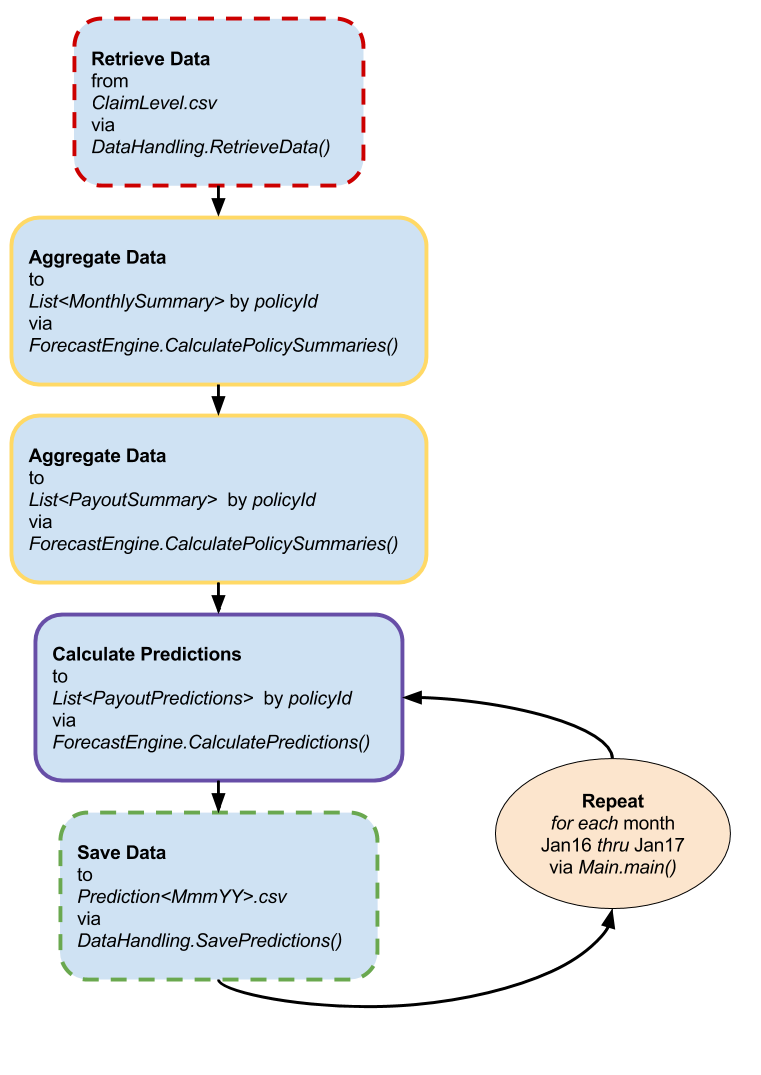
\includegraphics[scale=0.38]{payoutPredictionProcedure.png}
				\caption{A flow diagram of the procedure used to calculate predictions per policyId.}
				\label{fig:predProcedure}
			\end{figure}
			\FloatBarrier
					
			\subsubsection{Class Structures}
			The class structure of this computer model is rather simple. There are classes that encapsulate data structures used in calculations, and there are classes that encapsulate procedural functionality for implementing different algorithms. Outlined in the figure below is the general structure of the classes used in this computer model. The execution entry point in \emph{Main.main(String[] \emph{args})} uses classes from both the \emph{algorithms} and \emph{data} packages to implement the procedure outlined in the \emph{Procedure} (section \ref{sec:procedure}).
			\begin{figure}[!ht]
				\centering
				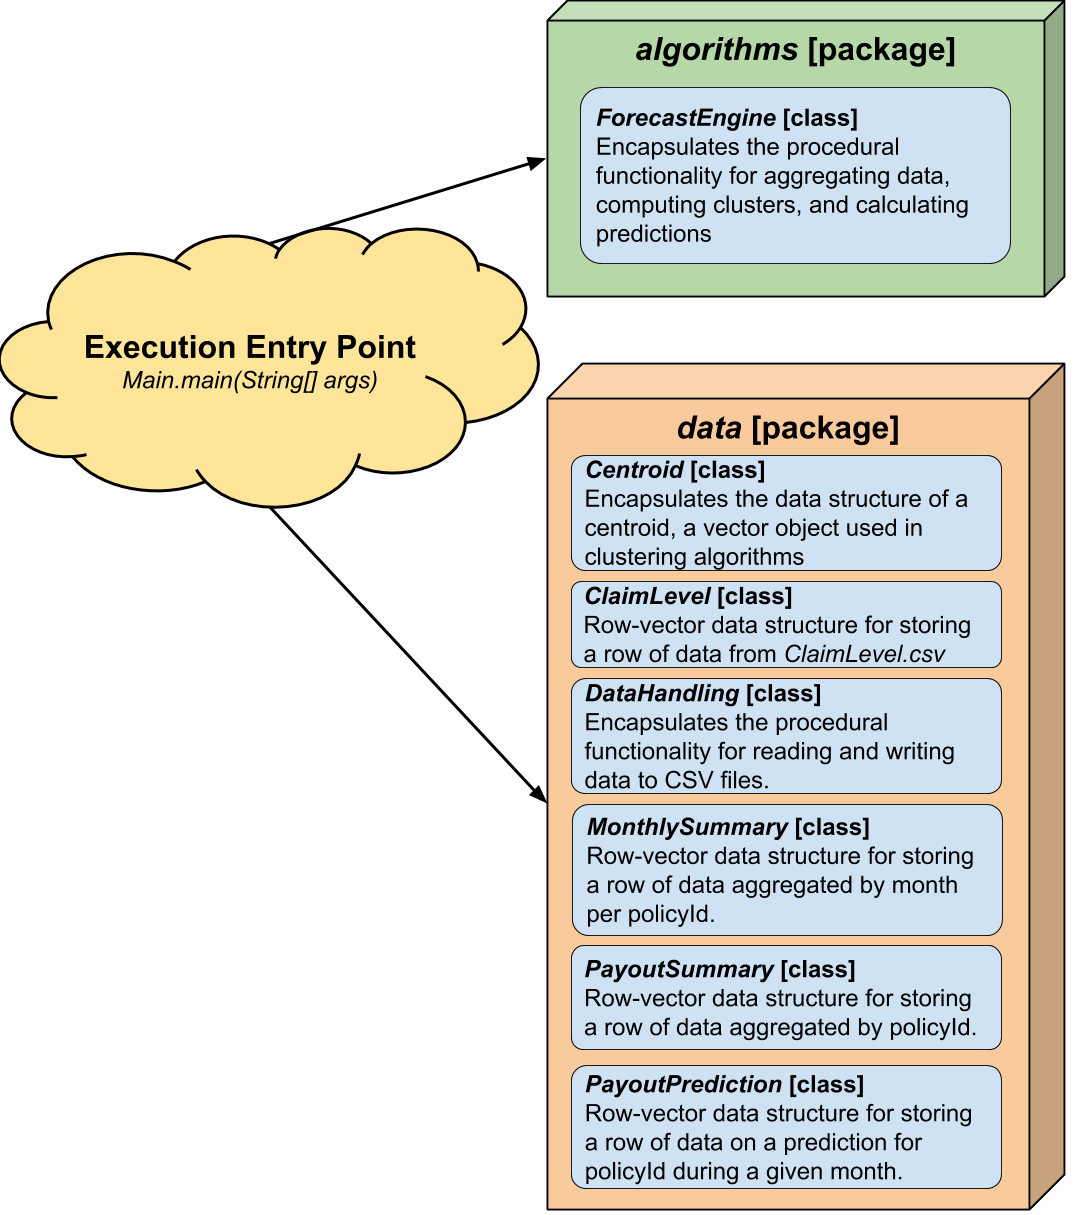
\includegraphics[scale=0.36]{classStructures.png}
				\caption{Above, is a general representation of the class structue used in this computer model. See \textbf{Javadoc}: \emph{/javadoc/index.html} for more detailed information.}
				\label{fig:classStructures}
			\end{figure}
			
\newpage		
		\subsection{Results}
		In order to determine how well this model performs, predictions were made not only for January 2017, but also for each month of claim level data found in \emph{ClaimLevel.csv}. Comparing the model's predictions with known results provides insight into how well the model predicts actual events. 
			
			\subsubsection{Predictions for January 2017}				
			\paragraph*{Analysis} 
			\subparagraph*{}The monthly payout predictions, forecasted for January 2017, are plotted below in Figure \ref{fig:jan17PredScat}. There are several similarities with an analog plot made from the 2016 claim level data in \emph{ClaimLevel.csv}, see Figure \ref{fig:amountByPolicyId_2016} below. Both of these plots fall within the same approximate quantile distribution: at least 25\% cost \$0,  50\% cost \$21.26 or less, 75\% cost \$73.97 or less, 95\% cost \$384.89 or less, and 99\% of all claims paid out in 2016 cost \$1494.30 or less. From the results emerging for the analysis of this initial computer, it appears this model is aptly predicting payout forecasts within this distribution. However, there is no way of knowing how well this model forecasts without comparing the actual results of amounts paid out on claims filed for January 2017 to the amounts predicted by this model. See the next section for further analysis into how well this initial model forecasts.
			
			\begin{figure}[!ht]
				\centering
				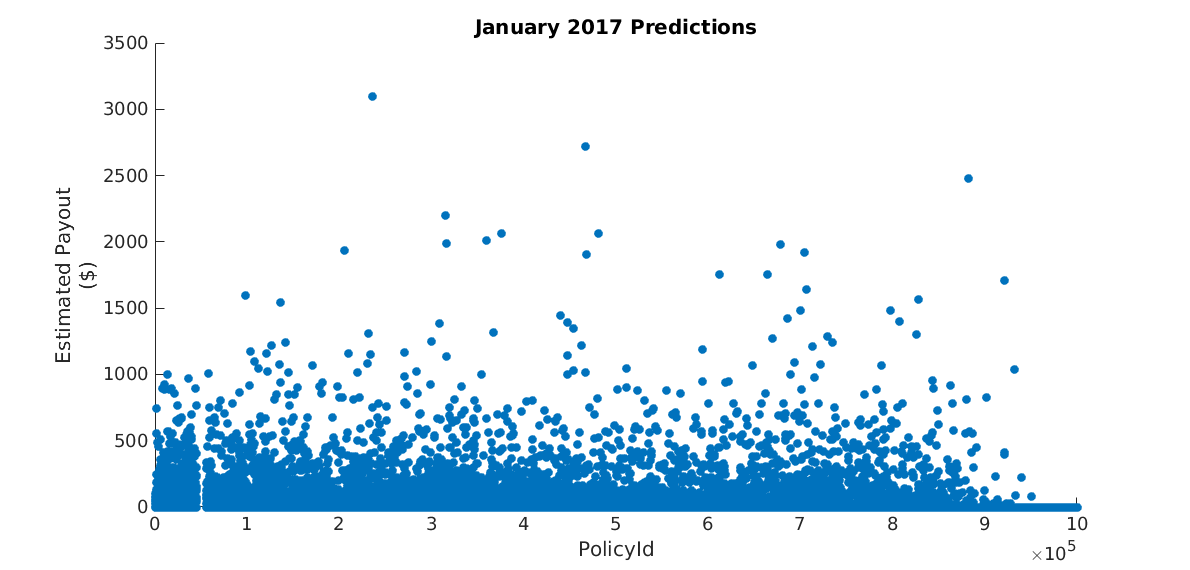
\includegraphics[scale=0.45]{jan17predictions.png}
				\caption{The predictions of estimated amount paid out on claims, by policy, for the month of January 2017. The total amount predicted for all claims paid out in January 2017 was \$844,382.61.
} 
				\label{fig:jan17PredScat}
			\end{figure}
			\FloatBarrier
			
			\begin{figure}[!ht]
				\centering
				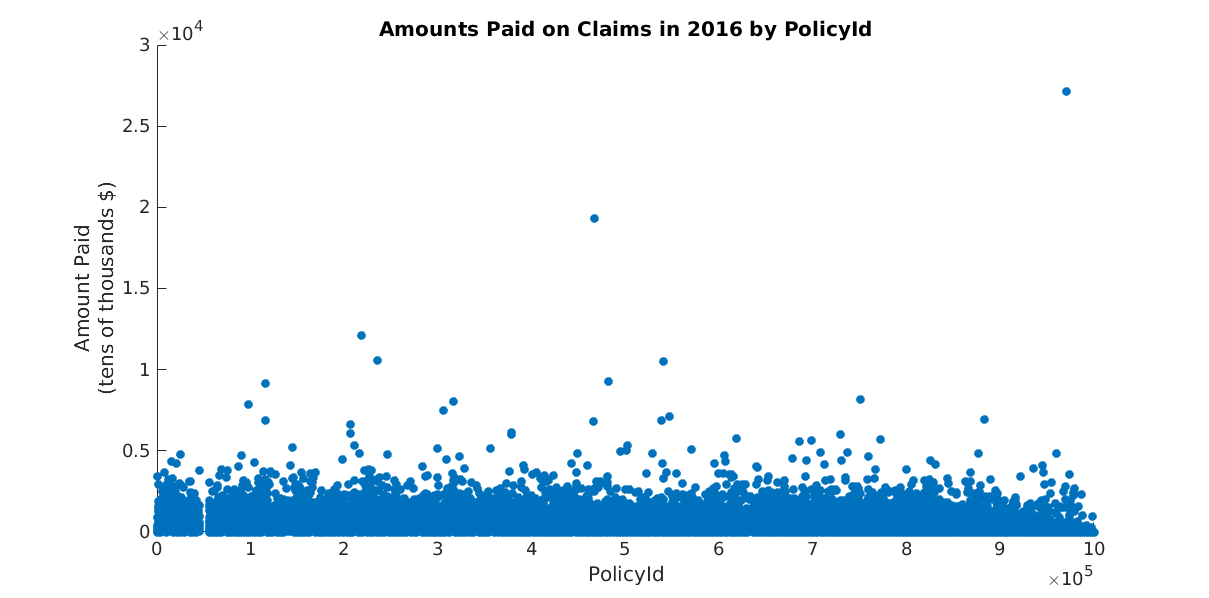
\includegraphics[scale=0.45]{amountByPolicyId_2016.png}
				\caption{The predictions of estimated amount paid out on claims, by policy, for the month of January 2017. The total amount predicted for all claims paid out in January 2017 was \$844,382.61.
} 
				\label{fig:amountByPolicyId_2016}
			\end{figure}	
			\FloatBarrier			
		
			\subsubsection{Predictions for Comparison} \label{sec:predComp}
			\paragraph*{Analysis} 
			\subparagraph*{}The ensuing analysis will delve into how this model's predictions compare to the actual amounts paid during 2016. Starting with Figure \ref{fig:actual_vs_model}, this graph shows a plot of the model's predictions in comparison to the actual amounts paid. Early in 2016 the model's predictions exceed the actual amounts paid by a very large margin. However, as more retrospective data is available for calculation, the model quickly becomes more accurate. By the time approximately six months of retrospective data, the model starts to predict within $\pm10\%$ of the actual amounts paid (see Figure \ref{fig:actual_vs_model_PE}). This level of accuracy continues for another 4-5 months, but by November and December of 2016, the model no longer predicts within $\pm20\%$ (see Figure \ref{fig:actual_vs_model_PE}).			
			\subparagraph*{}Notice that Figures \ref{fig:actual_vs_model}, \ref{fig:actual_vs_model_PE} only convey information about how the model predicted each month. To start understanding how well the model predicted for each policy, see Figure \ref{fig:actual_vs_model_meanPE}. Initally, at the beginning of 2016, the mean percent error measured per policy starts out very high, but as the year progresses, and more retrospective data is available for use in calculations, the mean percent error trends towards smaller values. To see suggestions for how to continue to drop this mean percent error per policy, see \emph{Further Work} (section \ref{sec:furtherWork}). In addition to using the mean percent error per policId to analyze the accuracy of this model, we must also use the standard deviation of this mean percent error per policyId to better understand how precise this model forecasts. From Figure \ref{fig:actual_vs_model_StDmeanPE} we see that for each month a forecast was made, the value of the standard deviation for mean percent error per policyId is very large. This implies that the precision of this model is relatively low. Additionally, there does not appear to be any outstanding trends or patterns in this distribution of data.
			
			\begin{figure}[!ht]
			\centering
				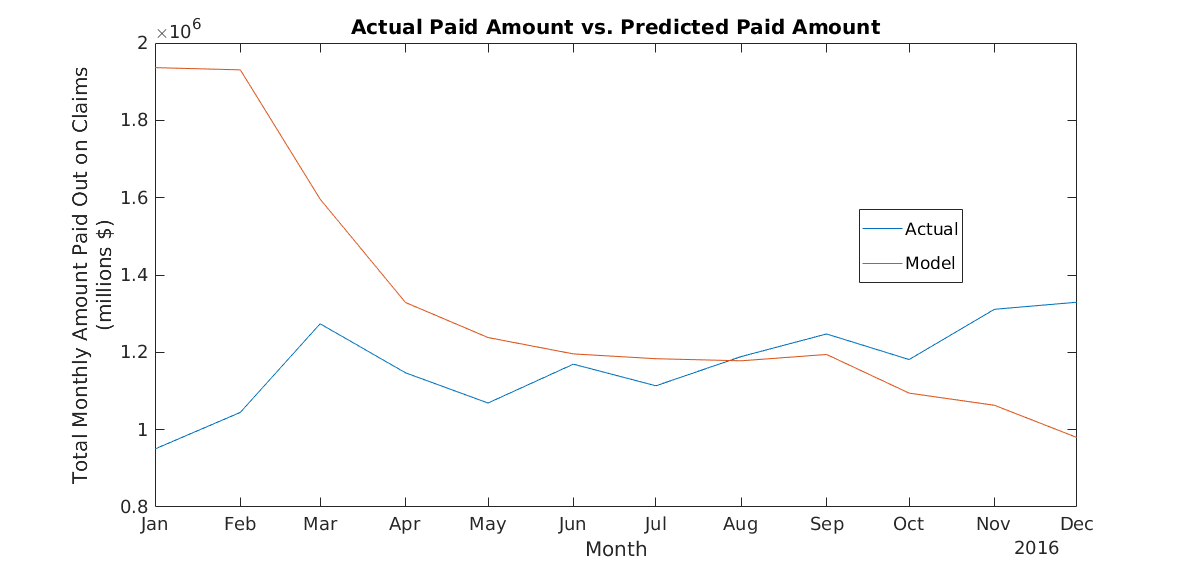
\includegraphics[scale=0.5]{actual_vs_model.png}
				\caption{The results from the forecasting model, aggregated by month (plotted in red), in comparison to the actual amounts paid on claims, also aggregated by month (plotted in blue).}
				\label{fig:actual_vs_model}
			\end{figure}
			\FloatBarrier
			
			\begin{figure}[!ht]
			\centering
				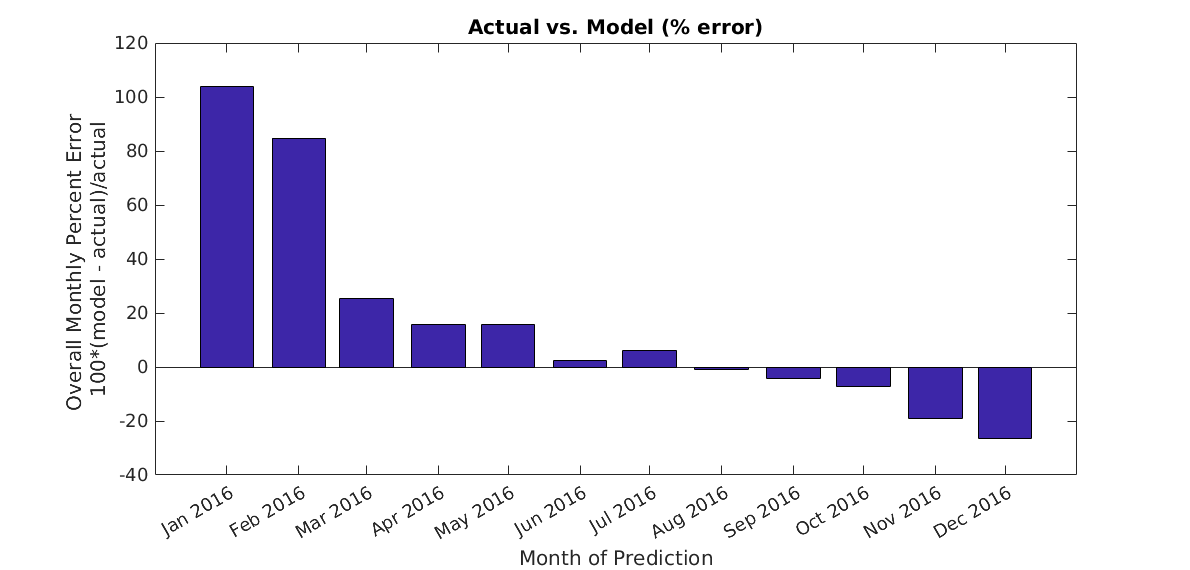
\includegraphics[scale=0.5]{actual_vs_model_PE.png}
				\caption{The percent error of the results from the forecasting model, aggregated by month, compared to the actual amounts paid out on claims per month during 2016.}
				\label{fig:actual_vs_model_PE}
			\end{figure}
			\FloatBarrier
			
			\begin{figure}[!ht]
			\centering
				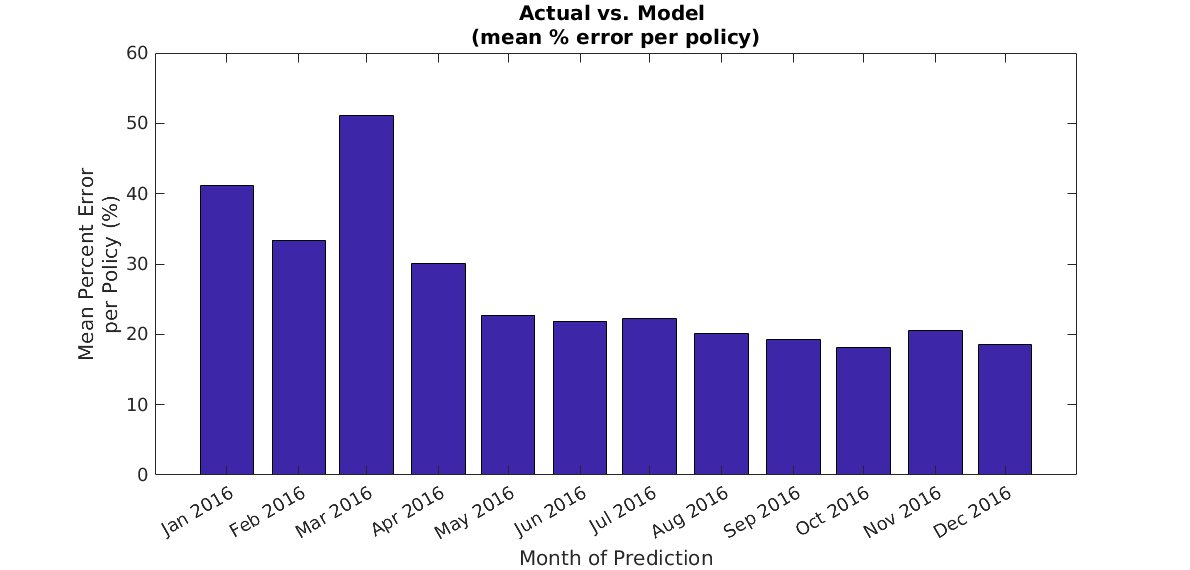
\includegraphics[scale=0.5]{actual_vs_model_meanPE.png}
				\caption{The mean percent error per policy, $p \in \mathbf{P}$, of the results from the forecasting model compared to the actual amounts paid out on claims per month during 2016.}
				\label{fig:actual_vs_model_meanPE}
			\end{figure}
			\FloatBarrier
			
			\begin{figure}[!ht]
			\centering
				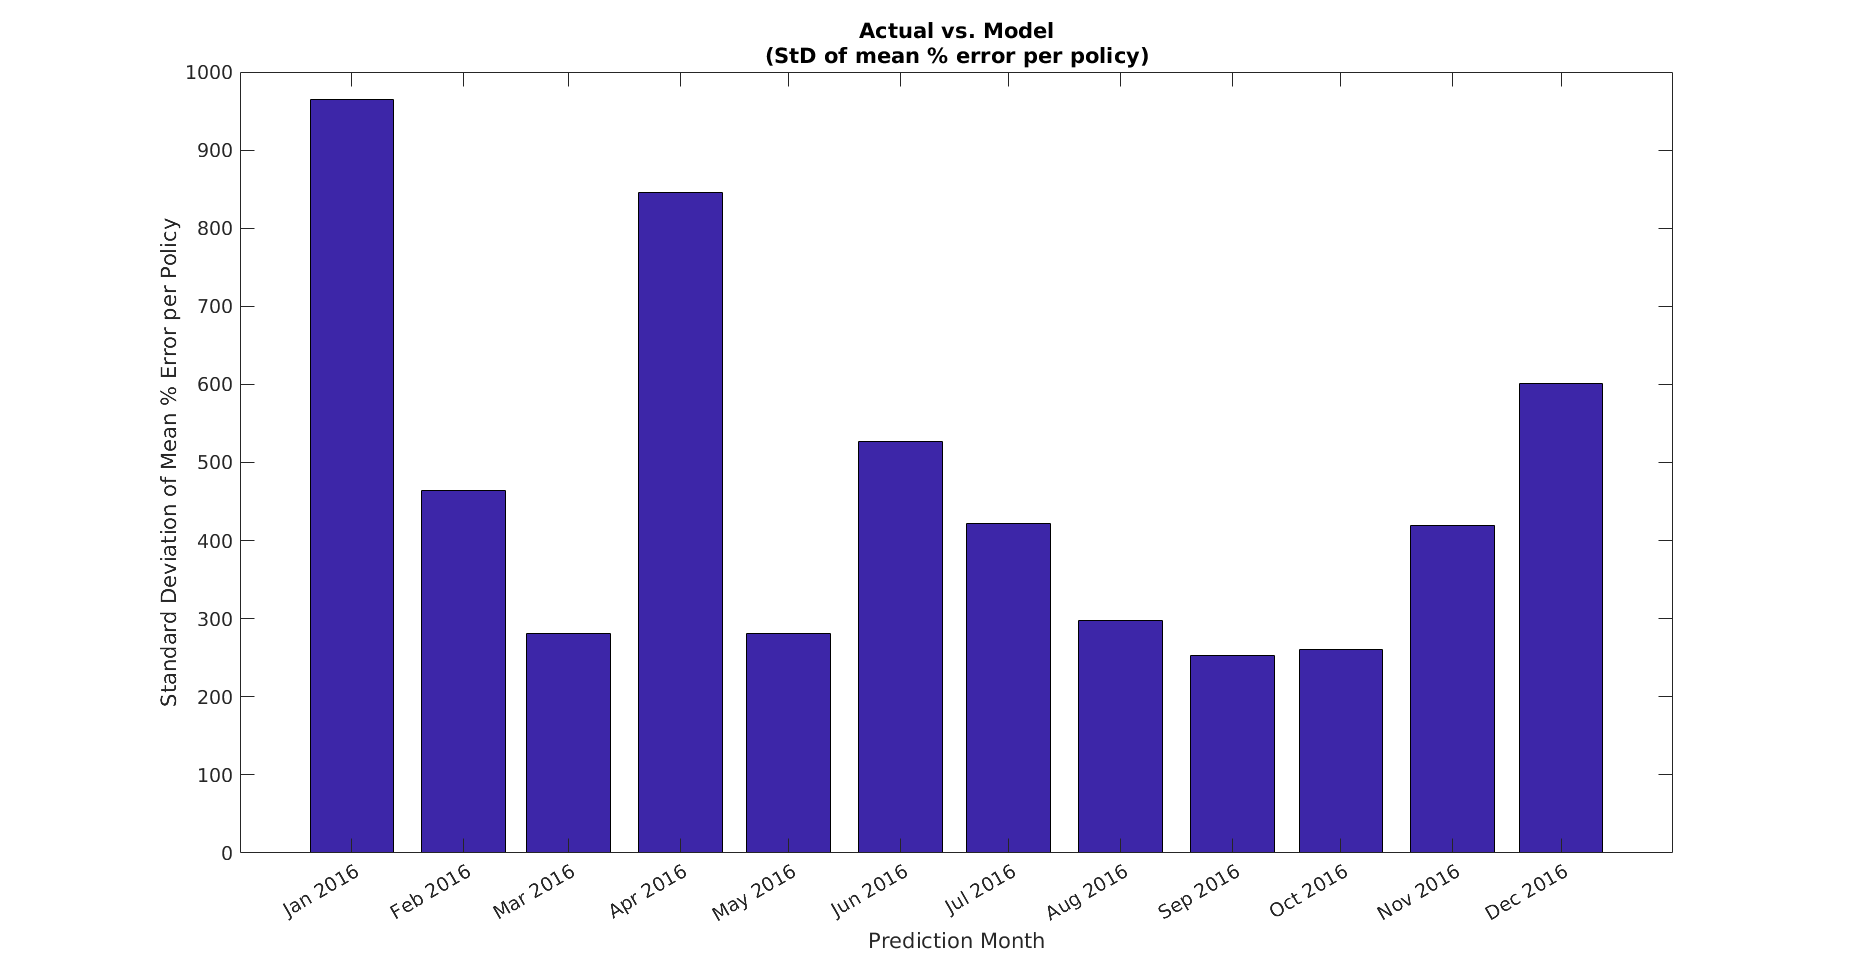
\includegraphics[scale=0.32]{actual_vs_model_StDmeanPE.png}
				\caption{The standard deviation of the mean percent error per policy, $p \in \mathbf{P}$, of the results from the forecasting model compared to the actual amounts paid out on claims per month during 2016.}
				\label{fig:actual_vs_model_StDmeanPE}
			\end{figure}
			\FloatBarrier
				
\newpage				
			\subsubsection{Application Profiling}\label{sec:appProfiling}
			
			\paragraph*{Analysis} 
			\subparagraph*{}The bar graph in Figure \ref{fig:total_time} shows, by prediction month, the total time it took to run the \emph{Procedure} (section \ref{sec:procedure}). Keep in mind that 1000 ms =  1 second, so, from this bar graph we can discern that the this program takes a most 2 second to run, but more often than not, the application takes only about a second to run. Due to the relatively simple calculations used in this model, and the relatively low volume of data, less than 5 MB in original \emph{ClaimLevel.csv}, this quick runtime is expected on any standard laptop. By adding the new features outlined in \emph{Further Work} (section \ref{sec:furtherWork}), to the original model, many of these features, especially a clustering algorithm, will significantly increase the runtime of the application. Running the application on a server, or other more computationally robust machine, will allow for the addition of these features with minimal slow downs.
						
			\begin{figure}[!ht]
			\centering
				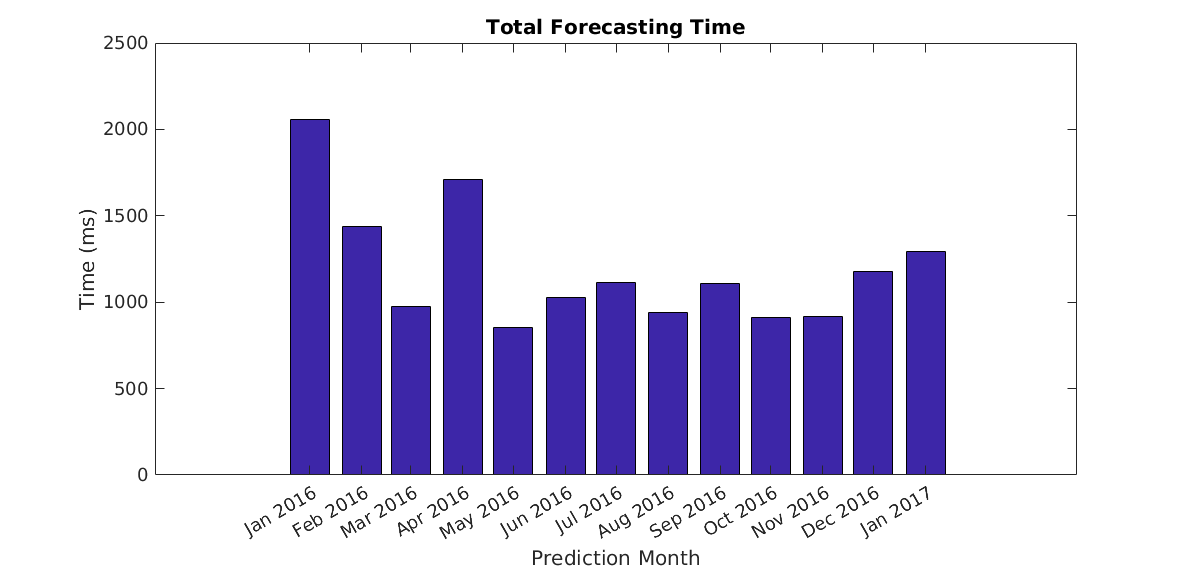
\includegraphics[scale=0.5]{total_time.png}
				\caption{The total time (in millisecconds) to retrieve data, calculate summaries, compute predictions, and save results, per month forecasted. Notice that application runtimes ranged between 850-2000ms (or 0.85-2.00 seconds), with a mean of 1194 ms (or 1.19 seconds).}
				\label{fig:total_time}
			\end{figure}
			\FloatBarrier
		
\newpage		
		\subsection{Conclusions}
		\paragraph*{}Now, to condense these results and analysis into some concluding remarks. First, a review of our original assumptions: periodic behavior, reversion to the mean, and diverse data (see section \ref{sec:assumptions}). In this initial model, periodic behavior and reversion to the mean were the main assumptions implemented, with little attention given to the diversity of defining characteristics of the data. The main reason for not making further use of the diversity of the data assumption is because there needs to be more dimensions of data for the clustering algorithm, that would have been implemented, to function properly. See \emph{Further Work} (section \ref{sec:furtherWork}) for more details on how this clustering algorithm would be implemented. 
		\paragraph*{}Returning back to reviewing the assumptions that were fully implemented: as seen in the \emph{Analysis} of the \emph{Predictions for Comparison} (section \ref{sec:predComp}), there is a lot of room for improvement with both the accuracy and precision of this model. With large margins of percent error across more than half the months predicted (see Figure \ref{fig:actual_vs_model_PE}), and across all policys (see Figure \ref{fig:actual_vs_model_meanPE}), the analysis of these results implies this model has inconsistent accuracy. Furthermore, for each month a prediction was made, the standard deviation of the percent error calculated per policy is very large (see Figure \ref{fig:actual_vs_model_StDmeanPE}), implying this model also has relatively low precision. Therefore, as a final forecasting model, this initial model fails quite spectacularly, but as a first draft this model provides all the neccessary framework to continue building a more accurate and precise forecasting model. See \emph{Further Work} (section \ref{sec:furtherWork}) for more details on how the equations in this model can be improved. Even though the analysis of these results implies this model has both low precision and low accuracy, this does not imply our assumptions of periodic behavior and reversion to the mean were falsely made. Rather, this low precision and low accuracy could imply that \emph{how} these assumptions were implemented must change first. Adding more dimensions of data, see \emph{Further Work} (section \ref{sec:furtherWork}), will open opportunities for new ways to implement a clustering algorithm, as well as improvements on the equations used for predictions (see equations \ref{eq:efmEq}, \ref{eq:tZscoreEq}, \ref{eq:timeProbEq}, \ref{eq:predEq}). While this initial model does an excellent job of laying the foundation and setting the framework for continued growth and expansion of this forecasting module, this initial model is not quite ready to be used for helping make decisions on behalf of the insurance company.
		\paragraph*{}As for the computer software, as an application, very little has been put to the test at this point. From the analysis of this application (section \ref{sec:appProfiling}), it is clear that this application runs very quickly. However, as explored next, in the \emph{Further Work} section, there will be a significant increase in both the amount of data being processed, and the number of computions used to calculate predictions, all of which will increase the runtime of the overal application significantly. Also as explored next in the \emph{Further Work} section, moving the application to a more robust computer (a server or computing cluster), will help mitigate these increases in runtime.		

\newpage						
		\subsection{Further Work} \label{sec:furtherWork}
		
		\subsubsection*{More Data (Dimensions)}
		More \emph{DATA}! Not just more rows of the same claim level data, but more \emph{dimensions} of data. This means information on any influential factors, such as the following:
			\begin{itemize}
				\item pet type (cat, dog, etc.)
				\item pet age (years, months)
				\item breed(s) (mixed, pure bred, etc.)
				\item most recent health info (weight, BMI(?), HR, blood pressure, body temperature, current ailments, etc.)
				\item any suggestions?
			\end{itemize}
			Being new to pet health insurance, it is hard to determine what factors can be used to predict. However, the more data there is to analyze, the better the models will be for forecasting amounts expected to pay in months or years to come.
		
		
		\subsubsection*{Changes to Equations} 
		With additional dimensions of data to analyze comes addititional opportunities for use in expanding the original set of equations (\ref{eq:efmEq}, \ref{eq:tZscoreEq}, \ref{eq:timeProbEq}, \ref{eq:predEq}). Until further access has been granted to more data, and until more analysis of this new data can be done, then more can be said about how these equations can be expanded. One possible avenue for changing the implementation of the reversion to the mean assumption (equation \ref{eq:predEq}), would be to use a variation of a PID algorithm. PID (Proportional, Integral, Differential) algorithms are used to control a feedback loop system such as the cruise control system in your car. The PID algorithm \emph{steers} the current measured status back towards the desired target value. For the purposes of this forecasting model, the desired target value would be the center (mean or median) of the cluster for each policy (see next section, \emph{Clustering Algorithm}). Originally, PID algorithms were mechanically implemented to steer naval and other maritime vessels onto a desired heading. Used in a wide variety of signal processing applications, PID algorithms remain a cornerstone for all of computer science. Check out the Wikipedia page for more general information about PID algorithms (https://en.wikipedia.org/wiki/PID\_controller).
		
			
		\subsubsection*{Clustering Algorithm}		
		With more data to analyze, the possibilities of using a clustering algorithm to group policies by similiar defining characteristics. Using a Birch clustering algorithm, with capabilities of processing enormous data sets, will allow for policies to be clustered into similar groups using a characteristic feature tree. Below is a glimpse into a possible set of clusterings based on the minimal data provided thus far. This snapshot was taken from a machine learning classification session in MATLAB\texttrademark. Continuing to expand the use of MATLAB\texttrademark\; with this model will be essential to leveraging the machine learning capabilities of clustering algorithms.  
		
			\begin{figure}[!ht]
				\centering
				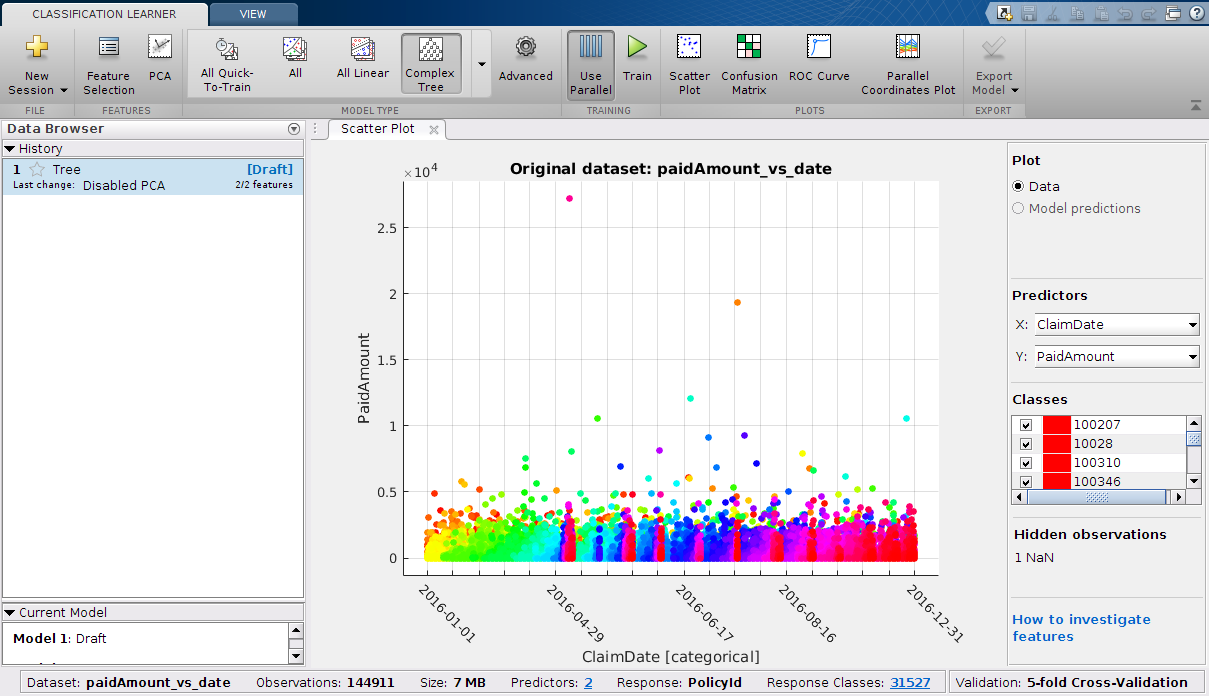
\includegraphics[scale=0.36]{Screenshot-MATLAB-clusterings.png}
				\caption{A glimpse into the possible clustering groups within the claim level data set from \emph{ClaimLevel.csv}. This is a screenshot from a machine learning classification session in MATLAB\texttrademark.}
				\label{fig:clusteringPotential}
			\end{figure}
			\FloatBarrier
		
		\subsubsection*{Database Connectivity} 
		Accessing more data, especially when adding more dimensions of data (as outlined above), will get computationally more exhausting if CSV files are continued as the only data persistence layer. To improve ease of use, and scale with increased computational use, using a database as the main data persistence layer will become neccessary. Reccomendations for using Microsoft SQL Server or Oracle's MySQL. Either way, a relational database strucure will be crucial. If a relational database structure already exists, 
		
		\subsubsection*{More Generalized Class Structure}
		The class structure that has been set forth thus far will scale appropriately, but there is room for great generalization in the class structure. Without bogging down on the techinal details, a more generalized structure will scale to larger applications even betterand will allow for greater flexibility in application.
		
		\subsubsection*{User Interface}
		Eventually, having access to this forecasting model, and all its variations, through a user interface will be useful for quickly comparing different settings across many models. This user interface should initially be a web interface, for ease of implementaion and access, but with options to migrate into a mobile and/or desktop app for simplicity and ease of use.

\end{document}